\documentclass[crop,tikz]{standalone}
\begin{document}
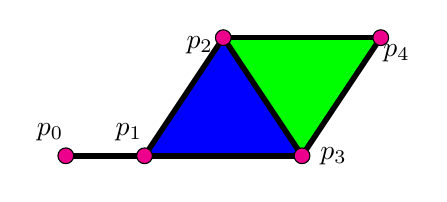
\begin{tikzpicture}
  \draw[fill=blue] (0,0) -- (2,0) -- (1,1.5);
  \draw[fill=green] (2,0) -- (1,1.5) -- (3,1.5);

  \draw[line width=2] (0,0) -- (-1,0);
  \draw[line width=2] (0,0) -- (1,1.5);
  \draw[line width=2] (0,0) -- (2,0);
  \draw[line width=2] (2,0) -- (1,1.5);
  \draw[line width=2] (1,1.5) -- (3,1.5);
  \draw[line width=2] (2,0) -- (3,1.5);

  \draw  (-1.2,.3) node{$p_0$};
  \draw[fill=magenta] (-1,0) circle (0.1);
  \draw (-.2,.3) node{$p_1$};
  \draw[fill=magenta] (0,0) circle (0.1);
  \draw (.7,1.4) node{$p_2$};
  \draw[fill=magenta] (1,1.5) circle (0.1);
  \draw (2.4,0) node{$p_3$};
  \draw[fill=magenta] (2,0) circle (0.1);
  \draw (3.2,1.3) node{$p_4$};
  \draw[fill=magenta] (3,1.5) circle (0.1);
\end{tikzpicture}
\end{document}
